% Nash equilibrium: the Rock Paper Scissors Lizard Spock tournament.
% Shared preamble for the write-on class slides.
%
% Every deck is designed to be projected and annotated live on a tablet:
% whatever takes time to draw is pre-drawn, and whatever the class produces is
% left blank. Compile a deck with `pdflatex main.tex` from its own directory,
% or run `make` in decks/ to build them all.
\documentclass[10pt]{article}

\usepackage[papersize={25.6cm,14.4cm}, margin=1.1cm, bottom=1.5cm,
            footskip=0.75cm]{geometry}
\usepackage[T1]{fontenc}
\usepackage[default]{sourcesanspro}
\usepackage{newtxsf}
\usepackage{tikz}
\usepackage{amsmath}
\usepackage{parskip}
\usepackage{fancyhdr}
\usetikzlibrary{arrows.meta, positioning, calc}

\setlength{\parindent}{0pt}

% Catppuccin Latte, the palette the course site uses in its light theme, so a
% deck on the projector looks like the pages the students read.
\definecolor{inkbg}{HTML}{EFF1F5}      % base
\definecolor{inksurface}{HTML}{E6E9EF} % mantle
\definecolor{inkfaint}{HTML}{CCD0DA}   % surface2, for rules and empty boxes
\definecolor{inktext}{HTML}{4C4F69}    % text
\definecolor{inkgrey}{HTML}{8C8FA1}    % overlay1, for anything secondary
\definecolor{inkblue}{HTML}{7287FD}    % lavender, the primary accent
\definecolor{inkteal}{HTML}{179299}    % teal
\definecolor{inkred}{HTML}{FE640B}     % peach, for whatever wants attention
\definecolor{inkmauve}{HTML}{8839EF}   % mauve

\pagecolor{inkbg}
\color{inktext}

% A box to write a number into. White against the tinted page, so it reads as
% somewhere to write rather than as part of the printed material.
\newcommand{\blank}[1][1.6]{%
  \tikz[baseline=(current bounding box.base)]{%
    \draw[inkfaint, line width=0.7pt, rounded corners=2pt, fill=white]
      (0,-0.18) rectangle (#1,0.62);}}

% A ruled area to work in. Faint dots keep handwriting level on a tablet.
\newcommand{\workspace}[2]{%
  \begin{tikzpicture}
    \draw[inkfaint, line width=0.7pt, rounded corners=3pt, fill=white]
      (0,0) rectangle (#1,#2);
    \foreach \gx in {0.5,1.0,...,#1}{%
      \foreach \gy in {0.5,1.0,...,#2}{%
        \fill[inkfaint] (\gx,\gy) circle (0.5pt);}}
  \end{tikzpicture}}

% A panel for material that is printed rather than written on.
\newcommand{\panel}[2]{%
  \begin{tikzpicture}
    \draw[inkfaint, line width=0.7pt, rounded corners=3pt, fill=inksurface]
      (0,0) rectangle (#1,#2);
  \end{tikzpicture}}

% An empty payoff grid. #1 is the list of action names, #2 is drawn afterwards
% so a page can add its own marks.
\newcommand{\payoffgrid}[2]{%
  \begin{tikzpicture}[scale=1.0, every node/.style={transform shape}]
    \foreach \name [count=\j from 0] in {#1}{%
      \node[font=\bfseries, text=inkblue] at (\j*2.7+1.35,0.55) {\name};
      \node[font=\bfseries, text=inkblue] at (-1.15,-\j*2-1) {\name};
      \foreach \k [count=\i from 0] in {#1}{%
        \draw[inkfaint, line width=0.7pt, fill=white]
          (\j*2.7,-\i*2) rectangle (\j*2.7+2.7,-\i*2-2);}}
    #2
  \end{tikzpicture}}

% The five actions on a pentagon. Each action beats the one next to it and the
% one across from it, so the two winning cycles are drawn as separate panels:
% ten labelled arrows on one diagram is a tangle nobody can read from the back
% of the room.
\newcommand{\rpslscycle}[3]{%
  \begin{tikzpicture}[scale=1.0, every node/.style={transform shape},
      >={Stealth[length=2.6mm]},
      action/.style={circle, draw=inkfaint, line width=1pt, fill=white,
                     text=inktext, minimum size=1.7cm, inner sep=1pt,
                     font=\small\bfseries},
      beats/.style={->, line width=1.2pt, shorten >=3pt, shorten <=3pt,
                    draw=#1},
      word/.style={font=\scriptsize, fill=inkbg, inner sep=1.6pt, text=#1,
                   sloped, pos=#2}]
    \foreach \name/\angle in {Rock/90, Lizard/18, Spock/-54,
                              Scissors/-126, Paper/162}{%
      \node[action] (\name) at (\angle:3.1) {\name};}
    \foreach \winner/\loser/\said in {#3}{%
      \draw[beats] (\winner) -- node[word] {\said} (\loser);}
  \end{tikzpicture}}

% Running header: the deck name on the left, the page's own step on the right.
% Each deck sets its name once with \deckname.
\newcommand{\deck}{}
\newcommand{\deckname}[1]{\renewcommand{\deck}{#1}}
\newcommand{\slidehead}[1]{%
  {\small\color{inkgrey}%
   \tikz[baseline=-0.5ex]{\fill[inkblue, rounded corners=1pt]
     (0,0) rectangle (0.22,0.22);}\;\deck
   \hfill \color{inkblue}\bfseries #1}\par
  {\color{inkblue}\rule{\linewidth}{1pt}}\par\vspace{0.35em}}

\pagestyle{fancy}
\fancyhf{}
\renewcommand{\headrulewidth}{0pt}
\fancyfoot[R]{\small\color{inkgrey}\thepage}

% Deck title pages, which carry no header and no page number.
\newcommand{\titleslide}[3]{%
  \thispagestyle{empty}%
  \begin{center}
    \vspace*{\fill}
    {\Huge\bfseries\color{inkblue} #1}\\[0.7em]
    {\LARGE\color{inkgrey} #2}\\[2.4em]
    #3
    \vspace*{\fill}
  \end{center}}

% One step of the plan on a title page.
\newcommand{\stepbox}[3]{%
  \node[draw=inkblue, line width=0.9pt, rounded corners=4pt, fill=white,
        minimum width=6cm, minimum height=1.7cm, align=center,
        text=inktext] (#1) at (#2,0) {#3};}


\deckname{Nash equilibrium}

\begin{document}

\titleslide{Nash equilibrium}{Rock Paper Scissors Lizard Spock, all the way down}{%
    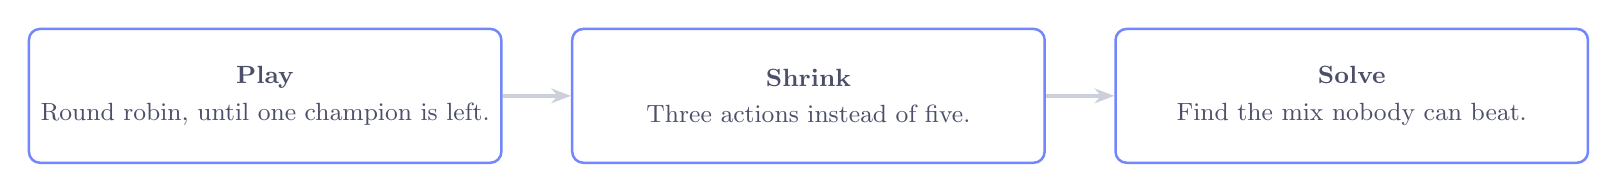
\begin{tikzpicture}[font=\small]
      \stepbox{s0}{0.0}{\textbf{Play}\\[0.25em]
                          Round robin, until one champion is left.}
      \stepbox{s1}{6.9}{\textbf{Shrink}\\[0.25em] Three actions instead of five.}
      \stepbox{s2}{13.8}{\textbf{Solve}\\[0.25em] Find the mix nobody can beat.}
      \draw[-{Stealth[length=2.5mm]}, inkfaint, line width=1.2pt] (s0) -- (s1);
      \draw[-{Stealth[length=2.5mm]}, inkfaint, line width=1.2pt] (s1) -- (s2);
    \end{tikzpicture}

    \vspace{2.4em}

    {\large Class champion: \blank[4] \hspace{1.6cm} Did I beat them? \blank[2]}}

\newpage
\slidehead{The rules}

\vspace{0.2cm}

\begin{minipage}[t]{0.47\linewidth}
\begin{center}
{\large\bfseries\color{inkteal} Beat the one beside you}\\[0.5em]
\rpslscycle{inkteal}{0.5}{Rock/Lizard/crushes, Lizard/Spock/poisons,
  Spock/Scissors/smashes, Scissors/Paper/cuts, Paper/Rock/covers}
\end{center}
\end{minipage}
\hfill
\begin{minipage}[t]{0.47\linewidth}
\begin{center}
{\large\bfseries\color{inkred} Beat the one across from you}\\[0.5em]
\rpslscycle{inkred}{0.24}{Rock/Scissors/crushes, Scissors/Lizard/decapitates,
  Lizard/Paper/eats, Paper/Spock/disproves, Spock/Rock/vaporises}
\end{center}
\end{minipage}

\vspace{0.4cm}

{\large Each action wins \blank[1.3], loses \blank[1.3] and draws
\blank[1.3]. So the game is \underline{\hspace{3.2cm}}, and every cell's
payoffs add to \blank[1.3].}

\newpage
\slidehead{Three actions, so we can see it}

\vspace{0.3cm}

\begin{minipage}[c]{0.52\linewidth}
\begin{center}
\payoffgrid{Rock, Paper, Scissors}{}
\end{center}
\end{minipage}
\hfill
\begin{minipage}[c]{0.44\linewidth}
{\large Fill in the \emph{row} player's payoff:}\\[0.8em]
{\large \hspace*{0.6cm} win $= +1$, \quad draw $= 0$, \quad lose $= -1$.}\\[1.6em]
{\large Then circle each player's best responses.}\\[1.6em]
{\large The column player's matrix is \blank[3.5].}
\end{minipage}

\vspace{0.4cm}

{\small\color{inkgrey} A cell with both players' best responses circled would be
a pure Nash equilibrium.}

\newpage
\slidehead{So there is no pure equilibrium}

\vspace{0.6cm}

{\large Whatever the pair of actions, somebody wants to move:}

\vspace{0.8cm}

\hspace{1cm}
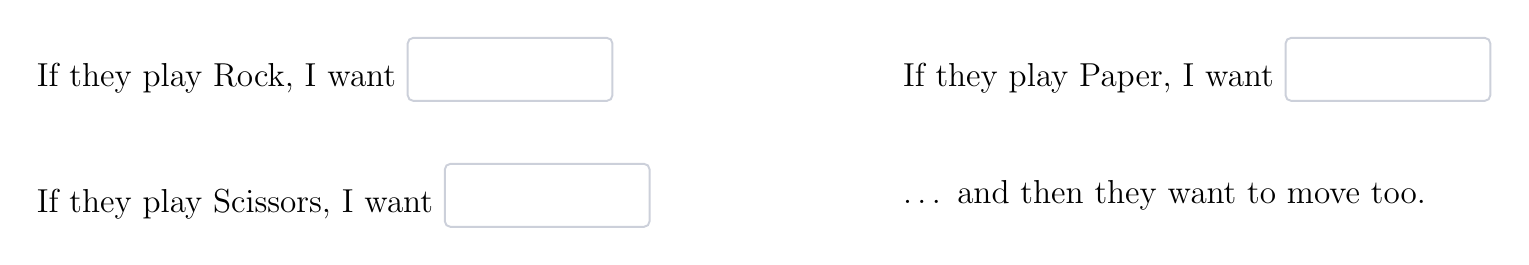
\begin{tikzpicture}[font=\large]
  \node[anchor=west] at (0,0)
    {If they play Rock, I want \blank[2.6]};
  \node[anchor=west] at (11,0)
    {If they play Paper, I want \blank[2.6]};
  \node[anchor=west] at (0,-1.6)
    {If they play Scissors, I want \blank[2.6]};
  \node[anchor=west] at (11,-1.6)
    {\ldots\ and then they want to move too.};
\end{tikzpicture}

\vspace{0.9cm}

{\large\bfseries So any equilibrium has to be
\underline{\hspace{4.5cm}}.}

\vspace{0.5cm}

\begin{center}
\workspace{22.6}{2.6}
\end{center}

\newpage
\slidehead{The best response condition}

\vspace{0.5cm}

{\large A mixed strategy \(\sigma\) is a best response to \(\tau\) if and only
if}

\vspace{0.6cm}

\begin{center}
\workspace{21}{3.4}
\end{center}

\vspace{0.9cm}

{\large In words: every action I actually use has to be
\underline{\hspace{6cm}}.}

\vspace{0.9cm}

{\large So if I mix over all three actions, all three must give me the same
expected payoff.}

\newpage
\slidehead{Making the other player indifferent}

\vspace{0.3cm}

{\large Suppose the column player uses
\(\sigma_c = (x, y, 1 - x - y)\) over (Rock, Paper, Scissors).}

\vspace{0.6cm}

\begin{minipage}[t]{0.52\linewidth}
{\large
\begin{tabbing}
\(u_r(\text{Scissors}, \sigma_c) \;=\;\) \= \kill
\(u_r(\text{Rock}, \sigma_c) \;=\;\) \> \blank[5.4]\\[1.5em]
\(u_r(\text{Paper}, \sigma_c) \;=\;\) \> \blank[5.4]\\[1.5em]
\(u_r(\text{Scissors}, \sigma_c) \;=\;\) \> \blank[5.4]
\end{tabbing}}
\end{minipage}
\hfill
\begin{minipage}[t]{0.44\linewidth}
{\small\color{inkgrey} Set them equal, and solve:}\\[0.4em]
\workspace{10.2}{5.2}
\end{minipage}

\vspace{0.8cm}

\begin{center}
{\Large \(\sigma_c \;=\;\) \blank[6]}
\end{center}

\newpage
\slidehead{How much work was that?}

\vspace{0.5cm}

{\large Support enumeration checks every pair of supports in turn.}

\vspace{0.9cm}

\hspace{1cm}
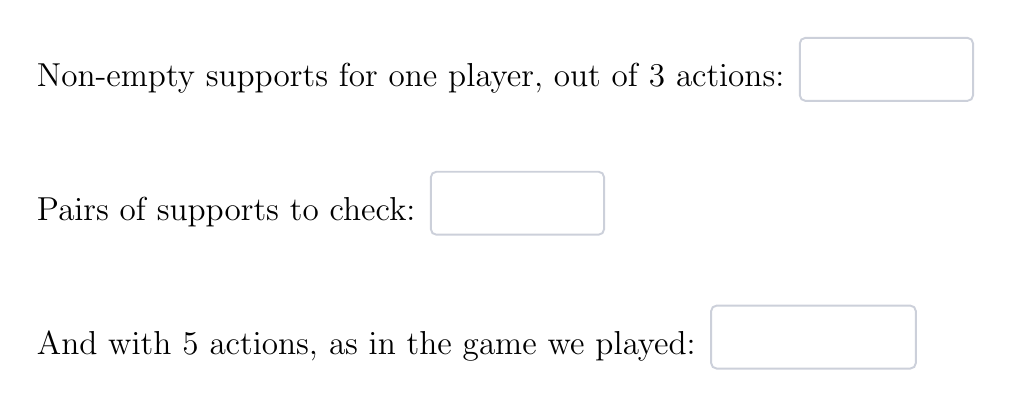
\begin{tikzpicture}[font=\large]
  \node[anchor=west] at (0,0)
    {Non-empty supports for one player, out of 3 actions: \blank[2.2]};
  \node[anchor=west] at (0,-1.7)
    {Pairs of supports to check: \blank[2.2]};
  \node[anchor=west] at (0,-3.4)
    {And with 5 actions, as in the game we played: \blank[2.6]};
\end{tikzpicture}

\vspace{1.4cm}

{\large\color{inkgrey} Which is why we want theorems, not enumeration.}

\newpage
\slidehead{The same thing, as an exam answer}

\vspace{0.5cm}

{\large What we just did in the room is \textbf{Question 1} on the Nash
Equilibrium page.}

\vspace{0.9cm}

\hspace{0.6cm}
\begin{minipage}{0.92\linewidth}
{\large
\begin{tabbing}
\hspace{1.2cm} \= \hspace{17cm} \= \kill
\textbf{(a)} \> Why it is symmetric and zero sum, and the column player's
  matrix. \> [3]\\[0.55em]
\textbf{(b)} \> Utilities for three given pairs of mixed strategies. \> [3]\\[0.55em]
\textbf{(c)} \> Use the best response condition to prove
  \((\tfrac13,\tfrac13,\tfrac13)\) is an equilibrium. \> [5]\\[0.55em]
\textbf{(d)} \> Prove it is the \emph{unique} equilibrium. \> [5]\\[0.55em]
\textbf{(e)} \> State and justify the equilibrium for the five-action
  game. \> [3]
\end{tabbing}}
\end{minipage}

\vspace{1.2cm}

\begin{center}
{\large\color{inkgrey} vknight.org/gt/topics/nash-equilibrium.html}
\end{center}

\end{document}
